\chapter{Fonctionalités}
Nous détaillerons dans cette partie les différentes fonctionalités que propose l'outil. Des exemples illustrés et des \dots  
%%%%%%%%%%%%%%%%%%%%%%%%%%%%%%%%%%%%%%%%%%%%%%%%%%%%%%%%%%%%%%%%%%%%%%%%%
\section{Histogrammes}
Type de diagramme répendu, l'histogramme fait partie des diagrammes que LoCD peut générer. L'exmple ci-dessus illustre un résultat basique avec la configure par défaut de LoCD soit : 
\begin{itemize}
\item
  Une unique couleur : bleu
\item
  Absence de titre, sous titre et notes
\item
  Représentation 2D
\end{itemize}

\begin{figure}[htbp]
  \centering
  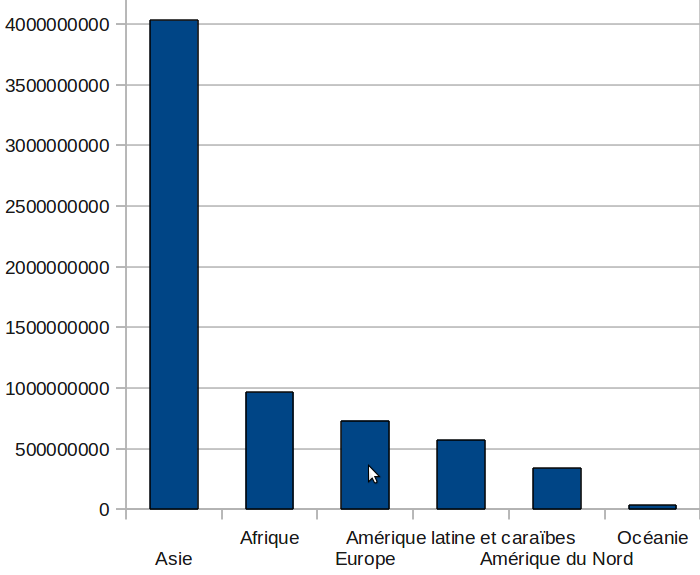
\includegraphics[scale=0.40]{img/diagrammebaton}
  \caption{Histogramme avec les paramètres par défaults}
  \label{fig:dbatons}
\end{figure}
Pour changer cette configuration par défault, se référer au chapitre configuration% références !!!!!!!!!!!!!!!!!!!!!!!!!!!!!!!!!!!!!!!!!!!!!!!!!!
%%%%%%%%%%%%%%%%%%%%%%%%%%%%%%%%%%%%%%%%%%%%%%%%%%%%%%%%%%%%%%%%%%%%%%%%%
\section{Diagrammes circulaires}
Appelés un diagramme « en camembert » (pie-chart en anglais pour sa forme en tarte), ce type de diagramme utilisé en statistiques. 
\begin{figure}[htbp]
  \centering
  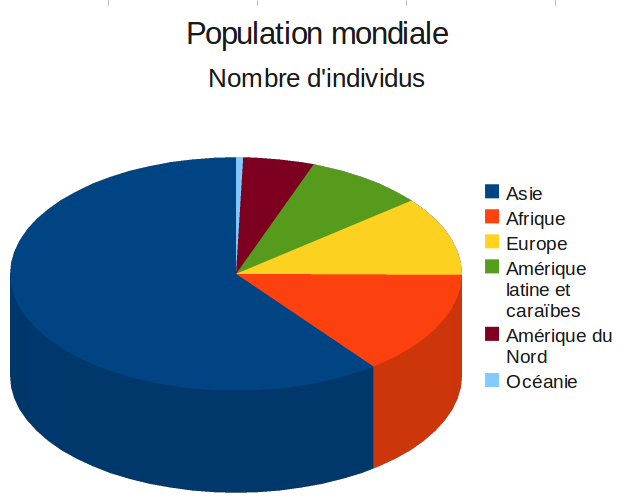
\includegraphics[scale=0.60]{img/diagrammecirculaire}
  \caption{Exemple avec un titre et un sous titre fournis dans les métas données.}
  \label{fig:dcirculaire}
\end{figure}
Sur cet exemple, plusieurs paramètres par défaut ont été modifiés. Les couleurs notamment. Pour apprendre comment effectuer un tel réglage se référer à la partie suivante : ~\ref{subsec:couleurs}
\clearpage
%%%%%%%%%%%%%%%%%%%%%%%%%%%%%%%%%%%%%%%%%%%%%%%%%%%%%%%%%%%%%%%%%%%%%%%%%
\section{Nuages de points}
Diagramme fréquement utilisée dans la représentation dans les séries statistiques à deux variables. LoCD permet de généger ce type de diagramme. L'exemple présenté dans la figure suivante, rassemble la plupart des fonctionalité que propose LoCD.
\begin{figure}[htbp]
  \centering
  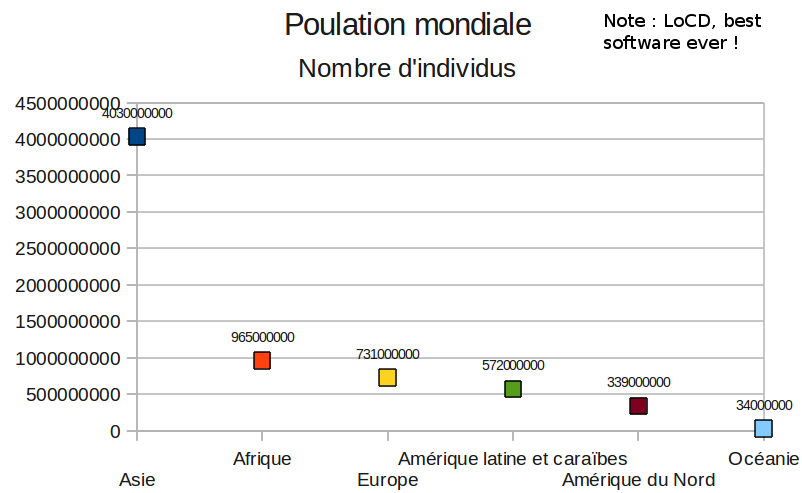
\includegraphics[scale=0.60]{img/diagrammenuages}
  \caption{Nuages de points avec toutes les méta données possibles renseignées}
  \label{fig:dnuages}
\end{figure}  
Les configuration en mode ligne de commandes sont détaillée dans ici : \ref{subsec:excom}.
